\documentclass{article}


\usepackage{amsmath,amssymb}
%\usepackage{dsfont} %install texlive-fonts-extra 
\usepackage{tikz}
\usetikzlibrary{bayesnet}

\author{Otto Fabius}
\title{Methods Intro}
\begin{document}

\maketitle




\section{Methods}

Our initial approach is to model topics using a VAE Approach such as Kingma \& Welling \cite{kingma2014Auto}. In this generative approach, we model the marginal probability $p(\mathbf{d})$ of a document with a softmax The graphical model is shown in Figure \ref{...}. Besides having continuous (Gaussian) latent variables in stead of binary latent variables, a notable difference with LDA \cite{bleiLDA} (see Figure \ref{VAE}) 
(and Deep Exponential Families?) 
is that we use document-level latent variables in stead of word-level latent variables. The documents are represented as word counts.
\\ (Mention why this choice is made and/or discuss pros/cons?) 

	\begin{figure}[ht]
		\begin{center}
			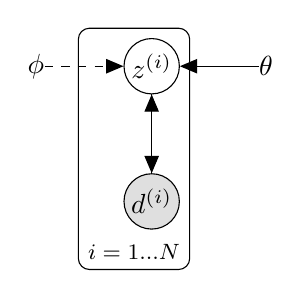
\begin{tikzpicture}[node distance = 1.5cm]
			
			
			\node[obs] (d) {$d^{(i)}$};
			
			\node[latent, above=of d] (z) {$z^{(i)}$};
			
			\node[const, right=of z] (th) {$\theta$} ;
			\node[const, left=of z] (ph) {$\phi$};
			
			
			\edge {z} {d};
			\edge {th} {z};
			\edge [dashed,bend left] {d} {z}
			\edge [dashed] {ph} {z}
			
			
			
			\plate {zd} {(z)(d)} {$i = 1...N$};
			
			\end{tikzpicture}
		\end{center}
		\caption{VAE Graphical Model}
		\label{VAE}
	\end{figure}

\subsection{Model details}

Both the encoder and the decoder are fully connected neural networks with ReLu activation functions. These may of course both be arbitrarily deep, but in the minimalistic case of one hidden layer in the encoder, we obtain the encoding \{$\mu^{(i)}, \log \sigma^{2(i)}$\} of the Gaussian latent variables from document $\mathbf{d}^{}(i)}$ as follows:

\begin{align}
content...
\end{align}

- encoder+decoder fully connected, ReLu everywhere, gaussian latent vars, softmax recon.

- objective function

- Adam (also future experiments)


\end{document}